\chapter{Implementation}
Here we should talk about bnfc and
alex. What we use from the differnet programs. How this is usefull
is it becouse of lazynes or are the existing solutions good??

\section{Alex}
Alex is a tool for generating lexical analysers built in Haskell, given a description of the language
in form of regular expressions. The result will be Haskell 98 compatible and can easly be used with the
parser Happy, a parser generator for Haskell.
\subsection{The DFA design}

\section{Monoid}
In abstract algebra a monoid is a set, $S$, and a binary operation $\bullet$ which furfills the following
three properties:
\begin{description}
\item[Closure] $\forall a,b \in S: a \bullet b \in S$
\item[Associativity] $\forall a,b,c \in S: (a \bullet b) \bullet c = a \bullet (b \bullet c)$
\item[Identity element] $\exists e \in S: \forall a \in S: e \bullet a = a \bullet e = a$
\end{description}

\subsection{The Basecase}
\subsection{The Conquer Step}

\section{Fingertree}
The incremental lexer uses a tree structure to save already lexed content.
This tree is of form Fingertree.
What that is and the basics of it is described in this section.

\subsection{Fundemental Conscepts}
Before describing the functionality, lets take a look on which buildingblocks
the fingertrees uses.
\paragraph{First,}
fingertrees uses monoids which has been described earlier in this chapter.
\paragraph{Second,} 
fingertrees uses Right and Left Reductions. This is a function which
collapses a structure of $f$ $a$ into a single value of type $a$. The basecase
for when the tree is empty is replaced with a constant value, such as 
$\emptyset$. Intermediate results are combined using a binary operation, like
the monoids $\bullet$. Reduction with a monoid always return the same value,
independent of the argument nesting. But for a reduction with an arbitraty
constant and binary operation there must be a specified nesting rule. If
combining operation are only nested to the right, or to the left, the obtained
result will be a skewed reductions, which can be singled out as a type class.
\lstinputlisting[language=Haskell]{examples/FingerTreeReduceFun.hs}

\subsection{Simple Sequence}
lets take a look on the definition on a 2-3 fingertree and how they can
implement a sequence. Lets start by looking at an ordinary 2-3 tree like in \cref{fig:2-3tree}.
\begin{figure}[!h]
  \centering
\tikzset{
  treenode/.style = {align=center, inner sep=0pt, text centered,
    font=\sffamily},
  branch/.style = {treenode, circle, draw=black, minimum size=0.2cm, text width=0.2em},
  leaf/.style = {treenode, circle, draw=black, font=\sffamily\bfseries, text width=1.5em}
}
    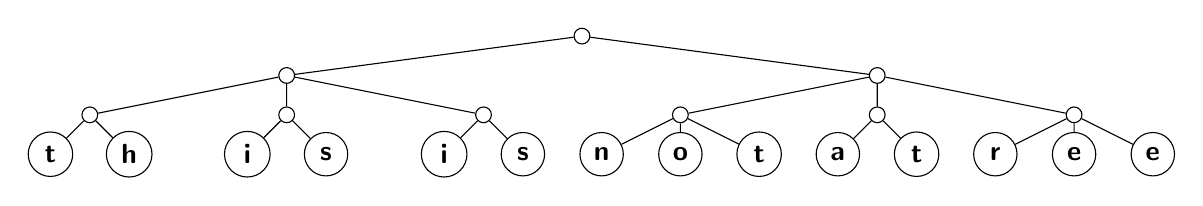
\begin{tikzpicture}[auto,
                        level 1/.style={sibling distance=7.5cm},
                        level 2/.style={sibling distance=2.5cm}, 
                        level 3/.style={sibling distance=1cm},
                        level distance = 0.5cm] 
\node [branch] {}
    child{ node [branch] {}
        child{ node [branch] {}
        	child{ node [leaf] {t}
            }
			child{ node [leaf] {h}
            }
        }
        child{ node [branch] {}
        	child{ node [leaf] {i}
            }
			child{ node [leaf] {s}
            }
        }
        child{ node [branch] {} 
        	child{ node [leaf] {i}
            }
			child{ node [leaf] {s}
            }
        }
    }
    child{ node [branch] {}
        child{ node [branch] {} 
        	child{ node [leaf] {n}
            }
			child{ node [leaf] {o}
            }
			child{ node [leaf] {t}
            }
        }
        child{ node [branch] {} 
        	child{ node [leaf] {a}
            }
			child{ node [leaf] {t}
            }
        }
        child{ node [branch] {} 
        	child{ node [leaf] {r}
            }	
			child{ node [leaf] {e}
            }
			child{ node [leaf] {e}
            }
        } 
    }
; 
\end{tikzpicture}
  \caption{Ordinary 2-3 tree
  \label{fig:2-3tree}}
\end{figure}
In this section the tree will store all data in the leafs. This can be expressed by defining an non-regular or nested type, as follows:
\lstinputlisting[language=Haskell]{examples/FingerTree2-3Tree.hs}
Operations on these types of trees usually takes logarithmic time in the size of the tree. 
But for sequence representations a constant time complexity is preferable for adding or removing element from the start or end of the sequence.

A finger is a structure which provides efficient access to nodes near the distinguished location. To obtain efficient access to the start and end of the sequence represented by the tree, there should be fingers placed at the left and right end of the tree. In the example tree, taking hold of the end nodes of and lifting them up together. The result should look like in \cref{fig:fingertree}
\begin{figure}[!h]
  \centering
  \tikzset{
  treenode/.style = {align=center, inner sep=0pt, text centered,
    font=\sffamily},
  branch/.style = {treenode, circle, draw=black, minimum size=0.2cm, text width=0.2em},
  blackbranch/.style = {treenode, draw,fill=black!33, minimum size=0.2cm, text width=0.2em},
  leaf/.style = {treenode, circle, draw=black, font=\sffamily\bfseries, text width=1.5em}
}
    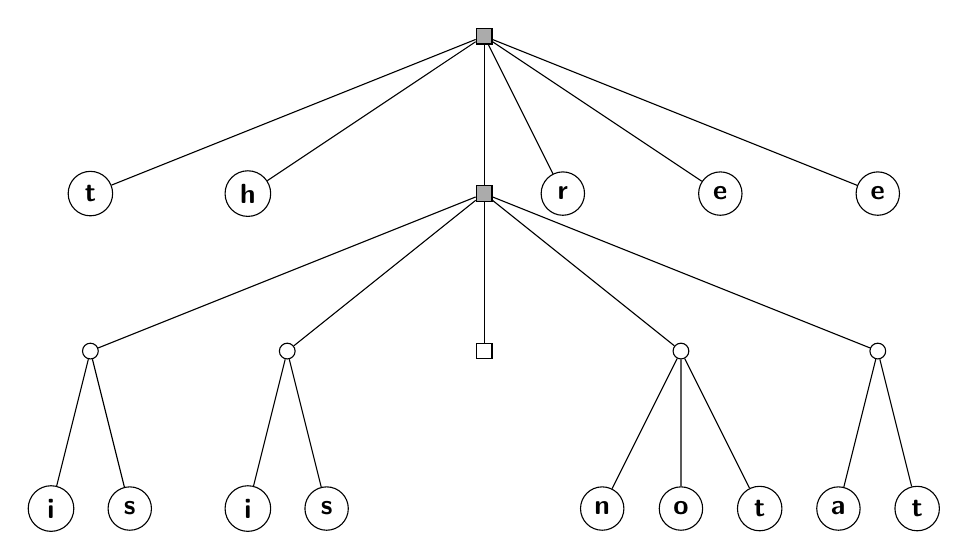
\begin{tikzpicture}[level distance=2cm, sibling distance = 2cm]
    \node[blackbranch] {} 
        child { node[leaf] {t} }
        child { node[leaf] {h} }
        child[level distance=2cm, sibling distance=2.5cm, grow=down] { node[blackbranch] {} [level distance=2cm]
            child { node[branch] {} [sibling distance=1cm]
                child { node[leaf] {i} }
                child { node[leaf] {s} }
            }            
            child { node[branch] {} [sibling distance=1cm]
                child { node[leaf] {i} }
                child { node[leaf] {s} }
            }
            child[level distance=2cm, grow=down] { node[blackbranch, fill=white] {}}
            child { node[branch] {} [sibling distance=1cm]
                child { node[leaf] {n} }
                child { node[leaf] {o} }
                child { node[leaf] {t} }
            }
            child { node[branch] {} [sibling distance=1cm]
                child { node[leaf] {a} }
                child { node[leaf] {t} }
            }
        }
        child { node[leaf] {r} }
        child { node[leaf] {e} }
        child { node[leaf] {e} }
    ;
  \end{tikzpicture} 
  \caption{2-3 Fingertree
  \label{fig:fingertree}}
\end{figure}

Since all leafs in the 2-3 tree where at the same level, the left and right spine has the same lenth. Therefor the left and right spines can be pair up to create a single central spine. Branching out from the spine is 2-3 trees. At the top level there are two to three elements on each side, while the other levels have one or two sub-trees, whose depth increases down the spine. Depending on if the root node had 2 or 3 branches in the original 2-3 tree, will the bottom node ether have a single 2-3 tree or empty. This structure can be described as follows:
\lstinputlisting[language=Haskell]{examples/HaskellFingerTree.hs}
Where Digit is a buffer of elements stored left to right, here represented as a list for simplicity

The non-regular definition of the $FingerTree$ type detemines the unusual shape of these trees, which is the key to there performance. The top level of the tree contains elements of type $a$. Next level contains elements of type $Node$ $a$. At the $n$th level, elements are of type $Node^n$ $a$. which are 2-3 trees with a depth of $n$. This will give that a sequence of $n$ elements is represented by a $FingerTree$ of depth $\Theta(\log n)$. Also an element at position $d$ from the nearest end is stored at a depth of $\Theta(\log d)$ in the $FingerTree$ \cite{fingertree}

\section{Sequences}
A sequence in Haskell is a form of sophisticated list. That is a list with better performance than the basic [] list notation. Where a list in Haskell has $\Theta(n)$ for finding, inserting or deleting elements, that is in a list there is only known current element and the rest of the list. Which will result in for example finding the last element of a list, the computer must look at every element until the empty list has been found as the rest of the list. Where in a sequence the last element can be obtained in $\Theta(1)$ time. Adding a element anywhere in the sequence can be done in worst case, $\Theta(log n)$ \cite{fingertree}. 

Since this project is about creating as real-time lexing tool, performance is very important. String in Haskell are just a list of characters, [Char], and therefor has $\Theta(n)$ in time cost. Lexing is working with strings in a high frequency and there for there is a idea of instead define a string as a sequence of characters instead of a list of character. 

\section{Transition Map}
\subsection{Array Format}
\subsection{Function Composition Format}
